%\VignetteIndexEntry{Using stm}
%\documentclass{article}
\documentclass[nojss]{jss}

\author{\hspace{1.1in}Margaret E. Roberts\\\hspace{1.1in}Harvard \And
  \hspace{1.5in}Brandon M. Stewart\\\hspace{1.5in}Harvard \And
  \hspace{1.5in}Dustin Tingley\\\hspace{1.5in}Harvard \And
}
\title{\pkg{stm}: \proglang{R} Package for Structural Topic Models}

\Plainauthor{Margaret E. Roberts, Brandon M. Stewart, Dustin Tingley} %% comma-separated
\Plaintitle{stm: R Package for Structural Topic Models} %% without formatting
\Shorttitle{Structural Topic Models}  %% a short title (if necessary)

\Abstract{
This vignette demonstrates how to use the Structural Topic Model, \pkg{stm}, \texttt{R} package. The Structural Topic Model (STM) allows researchers to estimate a topic model using information, metadata, about the documents. The \pkg{stm} package provides a range of features from model selection to extensive plotting and visualization options.
}

\Keywords{structural topic model, text analysis, LDA, \pkg{stm}, \proglang{R}}
\Plainkeywords{structural topic model, text analysis, LDA, stm, R} %% without formatting

\Address{
  Margaret E. Roberts\\
  Department of Government\\
  Harvard University\\
  1737 Cambridge St, Cambridge, MA, USA\\
  E-mail: \email{roberts8@fas.harvard.edu}\\
  URL: \url{http://scholar.harvard.edu/mroberts}\\
  \\
  Brandon M. Stewart\\
  Department of Government\\
  Harvard University\\
  1737 Cambridge St, Cambridge, MA, USA\\
  E-mail: \email{bstewart@fas.harvard.edu}\\
  URL: \url{http://scholar.harvard.edu/bstewart}\\
\\
  Dustin Tingley\\
  Department of Government\\
  Harvard University\\
  1737 Cambridge St, Cambridge, MA, USA\\
  E-mail: \email{dtingley@gov.harvard.edu}\\
  URL: \url{http://scholar.harvard.edu/dtingley}\\

}


% == BibTeX packages
\usepackage{natbib}

% == Other Packages
\usepackage{amsmath, amsfonts, amssymb, url, bm}
\usepackage{rotating}
\usepackage{latexsym}
\usepackage{graphicx}
\usepackage{ulem}

\usepackage{comment}


% == New Commands
% = For general typesetting
\newcommand\spacingset[1]{\renewcommand{\baselinestretch}{#1}\small\normalsize}
\renewcommand\r{\right}
\renewcommand\l{\left}

% = For bibtex
\def\citepos#1{\citeauthor{#1}'s (\citeyear{#1})}
\newcommand\citea{\citeauthor}

% = For general math
\newtheorem{theorem}{Theorem}[section]
\newtheorem{lemma}[theorem]{Lemma}
\newtheorem{corollary}[theorem]{Corollary}
\newtheorem{proposition}{Proposition}
\newtheorem{assumption}{Assumption}
\newcommand{\qed}{\hfill \ensuremath{\Box}}
\DeclareMathOperator*\argmax{argmax}
\DeclareMathOperator*\argmin{argmin}

% = For stats & econometrics
\renewcommand{\epsilon}{\varepsilon}
\newcommand\ud{\mathrm{d}}
\newcommand\dist{\buildrel\rm d\over\sim}
\newcommand\ind{\stackrel{\rm indep.}{\sim}}
\newcommand\iid{\stackrel{\rm i.i.d.}{\sim}}
\newcommand\logit{{\rm logit}}
\newcommand\cA{\mathcal{A}}
\newcommand\cN{\mathcal{N}}
\renewcommand\E{\mathbb{E}}
\newcommand\V{\mathbb{V}}
\newcommand\Cov{\textrm{Cov}}
\newcommand\Corr{\textrm{Corr}}
\newcommand\cJ{\mathcal{J}}
\newcommand\cT{\mathcal{T}}
\newcommand\y{{\bm y}}
\newcommand\X{{\bm X}}
\newcommand\x{{\bm x}}
\newcommand\eps{{\bm\varepsilon}}
\newcommand\zero{{\bm 0}}
\newcommand\be{{\bm\beta}}
\renewcommand\b{{\bm b}}
\newcommand\C{{\bm C}}
\newcommand\D{{\bm D}}
\newcommand\I{{\bm I}}
\newcommand\Z{{\bm Z}}
\newcommand\eeta{{\bm \eta}}
\DeclareMathOperator*\plim{plim}
\DeclareMathOperator\rank{rank}
\newcommand{\indep}{\mbox{$\perp\!\!\!\perp$}}
\DeclareMathOperator{\sgn}{sgn}
\def\independenT#1#2{\mathrel{\rlap{$#1#2$}\mkern2mu{#1#2}}}




\usepackage{Sweave}
\begin{document}
\Sconcordance{concordance:stmVignette.tex:stmVignette.Rnw:%
1 116 1 1 0 62 1 1 5 6 1 1 3 2 0 1 2 1 0 1 2 1 0 1 2 1 0 2 1 3 0 1 2 4 %
1 1 3 5 0 1 2 37 1 1 4 6 0 1 2 2 1 1 2 4 0 1 2 7 1 1 4 6 0 1 2 5 1 1 2 %
5 0 1 2 6 1 1 2 4 0 1 2 4 1 1 3 2 0 1 3 2 0 1 3 5 0 1 2 16 1 1 2 21 0 1 %
2 6 1 1 2 1 0 2 1 3 0 1 2 1 1 1 5 1 1 1 2 1 0 3 1 4 0 1 2 13 1 1 2 1 0 %
1 2 4 0 1 2 10 1 1 8 11 0 1 2 12 1 1 3 2 0 3 1 4 0 1 2 8 1 1 4 6 0 1 2 %
5 1 1 2 5 0 1 2 8 1 1 2 5 0 1 2 8 1 1 2 5 0 1 2 8 1 1 4 6 0 1 2 2 1 1 3 %
2 0 1 4 6 0 1 2 14 1 1 2 5 0 1 2 6 1 1 2 4 0 1 2 2 1 1 2 5 0 1 2 63 1 1 %
3 6 0 1 2 55 1}

\spacingset{1.5}

%%%%%%%%%%%%%%%%%%%%%%%%%%%%%%%%%%%%%%%%%%%%%%%%%%%%%%%%%%%%%%%%%%%%%%%%%%%%%%%%
\section{Introduction}
\subsection{Method Overview}

In this vignette we demonstrate how to use the Structural Topic Model, \pkg{stm}, \texttt{R} package.\footnote{We thank Jetson Leder-Luis, Christopher Lucas, and Alex Storer for various assistance in the construction of this package.  Additional details and development version at structuraltopicmodel.com} Building off of the tradition of generative topic models, such as the Latent Dirichlet Allocation \citep{blei2003latent} and Correlated Topic Model \citep{blei2007correlated}, the Structural Topic Model's key innovation is that it permits users to incorporate \emph{metadata}, defined as information about each document, into the topic model.

The goal of the Structural Topic Model is to enable the discovery of topics and the estimation of their relationship to document metadata. Outputs of the model can be used to conduct hypothesis testing about these relationships. Previous uses of the model span from the analysis of newspaper articles and their relationship to time and open ended responses in survey data. This vignette illustrates use of the various components of the package. The design of the package is such that users have a broad array of options to analyze the data and present findings utilizing a range of plotting tools.

\section{Estimation}
Like other topic models the STM is a generative model. That means we define a data generating process for each document and then use the data to find the most likely values for the parameters within the model.  The generative process for each document (indexed by $d$) can be summarized as:

\begin{enumerate}
\item Draw the document-level attention to each topic from a logistic-normal GLM based on document covariates $X_d$. \\
$\vec{\theta}_d | X_d\gamma, \Sigma \sim$ LogisticNormal$(\mu = X_d\gamma, \Sigma)$
\item Form the document-specific distribution over words representing each topic ($k$) using the baseline word distribution ($m$), the topic specific deviation $\kappa_k$, the covariate group deviation $\kappa_g$ and the interaction between the two $\kappa_i$.\\
$\beta_{d,k} \propto $ exp$(m + \kappa_{k} + \kappa_{g_d} + \kappa_{i=(kg_d)})$
\item For each word in the document, ($n \in 1, \dots, N_d$):
\begin{itemize}
\item Draw word's topic assignment based on the document-specific distribution over topics.\\
 $z_{d,n} | \vec{\theta}_d \sim $ Multinomial$(\vec{\theta})$
\item Conditional on the topic chosen, draw an observed word from that topic.\\
$ w_{d,n} | z_{d,n}, \beta{d,k=z} \sim $ Multinomial$(\beta_{d,k=z})$
\end{itemize}
\end{enumerate}

Regularizing prior distributions are used for $\gamma, \kappa$ and $\Sigma$ which help enhance interpretation and prevent overfitting. To fit the model, the Expectation-Maximization algorithm is used, given that we are estimating a set of latent variables. Further details are provided elsewhere \citep{nips2013,STMEdo,ajps,TextComparative}.\footnote{Available \href{http://scholar.harvard.edu/files/dtingley/files/topicmodelsopenendedexperiments.pdf}{here}, \href{http://scholar.harvard.edu/files/bstewart/files/stmnips2013.pdf}{here}, and \href{http://scholar.harvard.edu/files/dtingley/files/comparativepoliticstext.pdf}{here}.} In this vignette, we do not engage in interpretation of specific substantive results, and instead direct readers to the companion papers for discussion.


\section{Using the Structural Topic Model}

In this section we demonstrate the basics of using the package. Use of the STM typically proceeds in three key steps:
\begin{enumerate}
\item Tools for reading in and processing text data \\
(\code{textProcessor, readCorpus, prepDocuments})
\item Fitting the Structural Topic Model
(\code{stm, selectModel, manyTopics})
\item Plotting and inspecting results
(\code{plotModels},\code{plot.STM},\code{labelTopics}, \code{estimateEffect}, \code{plot.estimateEffect},\code{findThoughts}, \code{plotQuote})
\end{enumerate}

Next we walk through each of these steps to show users how to use the above functions. All of the functions come with help files, and examples, that can be accessed by typing ? and then the function's name.

\subsection{Reading in textual data}

The first step is to load data into \texttt{R}. Unlike standard quantitative text analysis techniques, textual analysis requires more preparation prior to analysis. In this section, we describe several different methods for loading data into \texttt{R} depending on the format of the textual data. These functions are provided in order to make the structural topic model as accessible as possible. A key aspect of this step for the \texttt{STM}, as compared to textual analysis using other techniques, is the need to make sure documents and their vocabularies are properly associated with their metadata.


\subsubsection{Reading in data from a ``spreadsheet''}

For purposes of example within the vignette, we will use a collection of blogposts about American politics that were written in 2008, from the CMU 2008 Political Blog Corpus \citep{poliblog}.\footnote{The set of blogs is available at \url{http://sailing.cs.cmu.edu/socialmedia/blog2008.html} and documentation on the blogs is available at \url{http://www.sailing.cs.cmu.edu/socialmedia/blog2008.pdf}.} The blogposts were gathered from six different blogs, American Thinker, Digby, Hot Air, Michelle Malkin, Think Progress, and Talking Points Memo.  Each blog has its own particular political bent.  The day within 2008 when each blog was written was also recorded.  Thus for each blogpost, there is metadata on the day written and the political ideology of the blog in which it was written.

A common way that researchers store textual data alongside covariates related to the text is by having all the data within one spreadsheet, with each row a separate observation and one of the column variables the ``textual'' data field. The \pkg{stm} packages comes with a special function, \code{textProcessor}, that conveniently reads in data stored in this format and processes the data to ready it for analysis in the \pkg{stm} package.  For example, users would first read in a csv file using native R functions, or load a pre-prepared dataframe as we do below. Next, they would pass this object through the \code{textProcessor} function. This function uses a range of features from the \texttt{tm} package, such as stemming and stop word removal.

\begin{Schunk}
\begin{Sinput}
> data <- read.csv("poliblogs2008.csv")
> data <- data[,-1] #removing row numbers
> processed <- textProcessor(data$documents, metadata=data)
> out <- prepDocuments(processed$documents, processed$vocab, processed$meta)
> meta<-out$meta
\end{Sinput}
\end{Schunk}

After reading in the data we suggest using the utility function \code{prepDocuments()} to process the loaded data to make sure it is in the right format. In particular, the \code{prepDocuments()} function properly associates metadata with textual data, re-indexes this relationship when textual data fields are blank, or become blank following pre-processing (such as with stop word removal). Please see the help file for this function for more details. It also removes infrequent terms, or too frequent terms, depending on user-set parameters. Importantly, \code{prepDocuments()} also will re-index all metadata/document relationships if any changes occur due to processing.

\subsubsection{Reading in data from other text processing programs}

The \code{readCorpus} function is helpful for reading in data produced in other text processing/analysis programs. The structure of these data sets are not the simple ``spreadsheet'' format like in the previous example.

For example, a program that is helpful for setting up and processing textual data, alongside document metadata, is \href{www.txtorg.org}{txtorg} \citep{TextComparative}. When using \pkg{txtorg}, three separate files are generated. A metadata file, a vocabulary file, and a file with the original documents. The function \code{readCorpus()} function can be called to help import this type of data, in order to import the vocabulary file from \texttt{txtorg} and set it up for analysis by the \texttt{stm} model. Please see the help file for this function for more details and additional options such as reading in data in Blei's LDA-C format.

Another way to load in data is to use data structured for use in other packages, like the popular \href{http://cran.r-project.org/web/packages/lda/}{LDA} package.

Here we load the political Blog Corpus from the LDA Package. Note that the LDA package only contains a subset of these blogs, and therefore the code below is just for showing how to load from Blei's LDA-C format.  We will be using the entire blog set for the rest of the examples.

\begin{Schunk}
\begin{Sinput}
> library(lda)
> data(poliblog.documents)
> data(poliblog.vocab)
> data(poliblog.ratings)
\end{Sinput}
\end{Schunk}


The LDA package uses a slightly different format for the vocabulary. Specifically it indexes words from 0 using the convention in C. We can convert this over to a more R-like 1-index using \code{prepDocuments()}, as well as perform other recoding options of metadata. Once again, the next step is to reassign the documents object from the output of \code{prepDocuments()} to its own object.

\begin{Schunk}
\begin{Sinput}
> poliblog.ratings <- as.factor(ifelse(poliblog.ratings == -100, 
+     "Liberal", "Conservative"))
> out <- prepDocuments(poliblog.documents, poliblog.vocab, poliblog.ratings)
> poliblog.documents <- out$documents
> poliblog.ratings <- out$meta
> poliblog.vocab <- out$vocab
\end{Sinput}
\end{Schunk}


After reading in and processing the textual data, it is important to inspect features of the documents and the associated vocabulary list. If users encounter problems with estimation, they should always inspect features such as these, and if using metadata, make sure the metadata has the same number of rows as there are documents. Furthermore, the model does not permit estimation when there are variables used in the model that have missing values.

Matt Taddy's \pkg{textir} package uses a corpus in another format which is drawn from \citet{gentzkow2010drives}. This corpus contains 1000 phrases from the 2005 Congressional record. Each ``document'' is a different legislator's transcript for that year. To read in the data we use the \code{readCorpus()} function specifying the type as \code{Matrix} because the data is stored as a sparse matrix from the \code{Matrix} package. This gives us our document-term matrix, vocabulary, and metadata.

\begin{Schunk}
\begin{Sinput}
> library(textir)
> data(congress109)
> temp <- readCorpus(congress109Counts, type="Matrix")
> documents.gs <- temp$documents
> vocab.gs <- temp$vocab
> metadata.gs <- congress109Ideology #this is our metadata.
> out <-prepDocuments(documents.gs, vocab.gs, metadata.gs)
> documents.gs <- temp$documents
> vocab.gs <- temp$vocab
> metadata.gs <- out$meta
> rm(temp)
\end{Sinput}
\end{Schunk}


\subsection{Estimating the STM}

Once data is properly imported there will be documents, vocabulary and metadata that can be used for an analysis. In this subsection we illustrate how to estimate the STM.\footnote{We note that all the examples here have a very small number of maximum iterations of the EM algorithm to reduce run time, and so no substantive conclusions should be drawn.}

\subsubsection{Ways to use metadata}

Typically, metadata about documents has not been incorporated into the topic model. The key innovation of the STM is to incorporate metadata in the the analysis. In the STM there are two ways metadata about each document can be included in the model: topical prevalence and topical content.  Metadata covariates for \emph{topical prevalence} allow the observed metadata to affect the frequency with which a topic is discussed.  Covariates in \emph{topical content} allow the observed metadata to affect the word rate use within a given topic, that is, how a particular topic is discussed. We first show how to leverage metadata for understanding topical content.

\subsubsection{Estimation with topical prevalence parameter}

In this example, we use the ratings variable (blog ideology) as a covariate in the topic \emph{prevalence} portion of the model with the CMU Poliblog data described above. Each document can be a mixture of multiple topics. Topical prevalence captures how much each topic contributes to a document. Because different documents come from different sources, it is natural then to want to allow this prevalence to vary with metadata that we have about document sources.

In this example we simply let prevalence be a function of the ``ratings'' variable, which is coded as either ``Liberal'' or ``Conservative.'' Here a five topic STM is estimated. The output from the model, poliblogPrevFit, could then be passed through the various functions we discuss below for inspecting the results. If a user wishes to specify additional prevalence covariates, they would do so using the standard formula notation common in R which we discuss at greater length below.

\begin{Schunk}
\begin{Sinput}
> poliblogPrevFit <- stm(out$documents,out$vocab,K=20,
+             prevalence =~ rating, max.em.its=75, data=meta)
> 
\end{Sinput}
\end{Schunk}

For example purposes only, the model is set to run for a maximum of 74 EM iterations.  Typically, convergence of the model will be monitored by the change in the approximate bound between EM iterations.  Once the bound has a small enough change between iterations, the model is considered converged. To reduce compiling time, in this vignette we do not run the models and instead load a workspace with the models already estimated.

\begin{Schunk}
\begin{Sinput}
>  load(url("http://dl.dropboxusercontent.com/u/12848660/ModelObjectsSTMFinal.RData"))
\end{Sinput}
\end{Schunk}

\subsection{Model Selection}

As with all mixed-membership topic models the posterior is intractable and non-convex, resulting in a multimodal estimation problem which can be sensitive to initialization. Hence users may wish to estimate a many models, each from randomly generated starting values, and then evaluate each model according to some separate standard. The function \code{selectModel} automates this process to facilitate finding a model with good properties.

Users specify the number of ``runs'', which in the example below is set to 10. \code{selectModel} first first casts a net where ``run'' (below 10) models are run for two EM steps, and then models with low likelihoods are discarded. Next the default returns the 20\% of models with the highest likelihoods which are then run until convergence or the EM iteration maximum is reached. Notice how that options for the \code{stm()} function can be passed, such as \code{max.em.its}. If users would like to select a larger number of models to be run completely, this can also be set with an option specified in the help file for this function.

\begin{Schunk}
\begin{Sinput}
> poliblogSelect <- selectModel(out$documents,out$vocab,K=20,
+         prevalence =~ rating, max.em.its=j, data=meta,runs=10)
> 
\end{Sinput}
\end{Schunk}

In order to select a model for further investigation, users must choose from one of the candidate models output from \code{selectModel()}. To do this \code{plotModel()} can be used to plot the average \emph{semantic coherence} and \emph{exclusivity} scores for each topic (represented by topic numbers) as well as the semantic coherence and exclusivity for each topic.\footnote{See \citet{STMEdo,ajps} for a discussion of these criteria.} Each of these criteria are calculated for each topic within a model run. The \code{plotModel()} function calculates the average across all topics for each run of the model and plots these by labeling the model run with a numeral. Often times users will select a model with desirable properties in both dimensions (i.e., models with average scores towards the upper right side of the plot). As shown in Figure~\ref{fig:select}, the \code{plotModel()} function also plots each topic's values which helps give a sense of the variation in these parameters.\footnote{The utility function \code{manyTopics()} allows the user to specify a range of topic numbers that they would like to run \code{selectModel} on. Please consult the help file for information on this function. Especially note that the process of extracting results differs from \code{selectModel}.}


\begin{figure}[t!]
\begin{center}
\begin{Schunk}
\begin{Sinput}
> plotModels(poliblogSelect)
\end{Sinput}
\end{Schunk}
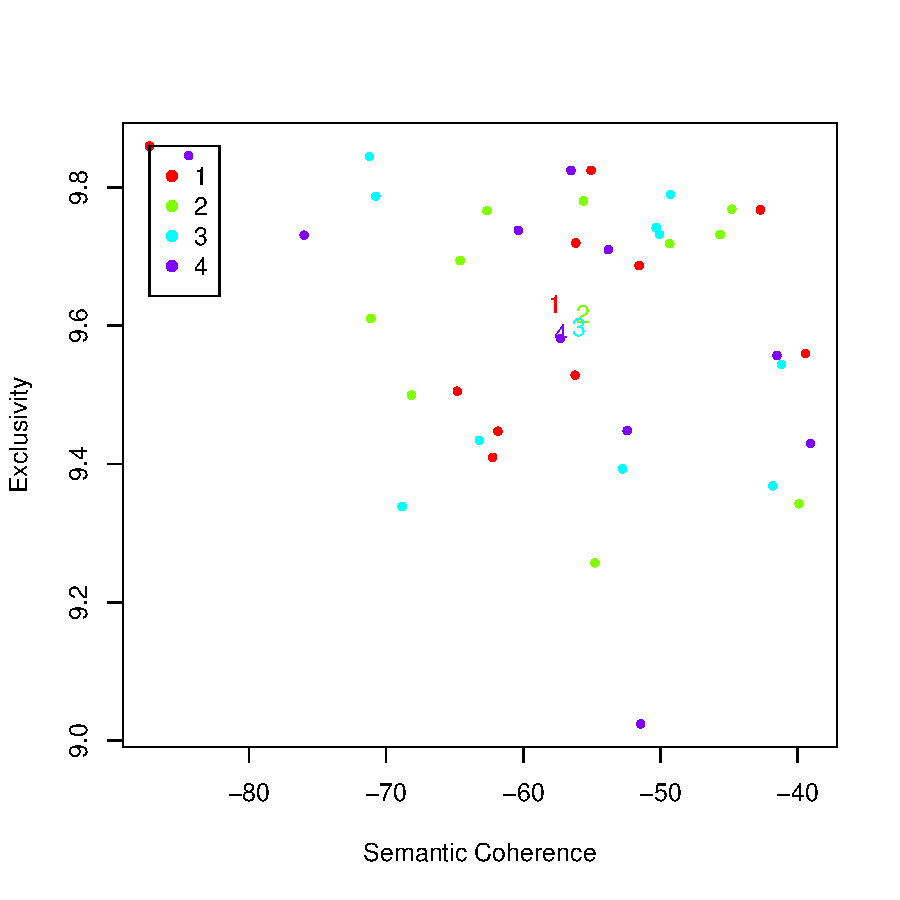
\includegraphics{stmVignette-009}
\caption{Plot of selectModel results.}
\label{fig:select}
\end{center}
\end{figure}


\subsection{Interpreting the STM: Plotting and inspecting results}

After estimating a choosing a model based on ex-ante criteria, the task of interpretation comes next which is especially crucial for any unsupervised procedure. There are many ways to investigate the output, ranging from inspecting the words associated with topics to the relationship between metadata and topics. To investigate the output of the model the \pkg{stm} package provides a number of options.
\begin{enumerate}
\item Displaying words associated with topics (\code{labelTopics},\code{plot.stm(,type="labels")}) or documents highly associated with particular topics (\code{findThoughts},\code{plotQuote})
\item Plotting relationships between metadata and topics/topical content (\code{estimateEffect}, \code{plot.estimateEffect})
\item Corpus level summaries (\code{plot.topicCorr},\code{plot.stm(,type="summary")})
\end{enumerate}

\subsubsection{Exploring Topics}

We next describe two ways that users can explore the topics that have been estimated. The first way is to look at collections of words that are associated with topics. In the second way is to read actual documents that are estimated to be highly associated with each topic. Both of these ways should be used.

To explore the words associated with each topic we can use the \code{labelTopics()} function. This will print to the monitor words associated with each topic. The function by default prints several different types of word profiles, including highest probability words and FREX words.\footnote{For more information on FREX and high probability rankings, see \citet{nips2013,STMEdo,ajps,TextComparative}. For more information on score, see the LDA R package, \url{http://cran.r-project.org/web/packages/lda/lda.pdf}. For more information on lift, see \citet{taddy2012multinomial}.}  In order to translate these results to a format that can easily be used within a paper, the \code{plot.stm(,type="labels")} function will print topic words to a graphic device. Notice that in this case, the labels option is specified as the \code{plot.stm} function has several functionalities.

\begin{Schunk}
\begin{Sinput}
> labelTopics(poliblogPrevFit,topics=c(1,3))
\end{Sinput}
\begin{Soutput}
Topic 1 Top Words:
 	 Highest Prob: will, women, one, school, life, live, year 
 	 FREX: school, women, film, children, men, life, young 
 	 Lift: film, girl, music, hollywood, mother, daughter, father 
 	 Score: film, women, school, children, famili, student, parent 
Topic 3 Top Words:
 	 Highest Prob: senat, democrat, bill, republican, vote, hous, legisl 
 	 FREX: legisl, bill, congression, committe, pelosi, senat, reid 
 	 Lift: reid, pelosi, legisl, nanci, congression, veto, bipartisan 
 	 Score: senat, legisl, republican, vote, democrat, bill, congress 
\end{Soutput}
\end{Schunk}

To read documents that are highly associated with topics the \code{findThoughts} function can be used. This function will print to the user the documents highly associated with each topic.\footnote{The \code{theta} parameter in the stm object output has the posterior probability that this function uses.} In this example, for expositional purposes, we restrict the length of the documents to just plot the first 250 characters. When users would like longer examples, native R graphics commands can be used to enlarge the graphic device. To print example documents to a graphics device \code{plotQuote} can be used. The results are displayed in Figure~\ref{fig:example}).

\begin{Schunk}
\begin{Sinput}
> k<-findThoughts(poliblogPrevFit, texts=shortdoc,  n=2, topics=5)$docs[[1]]
\end{Sinput}
\end{Schunk}

\begin{figure}[t!]
\begin{center}
\begin{Schunk}
\begin{Sinput}
> plotQuote(k, width=60, main="Topic 5")
\end{Sinput}
\end{Schunk}
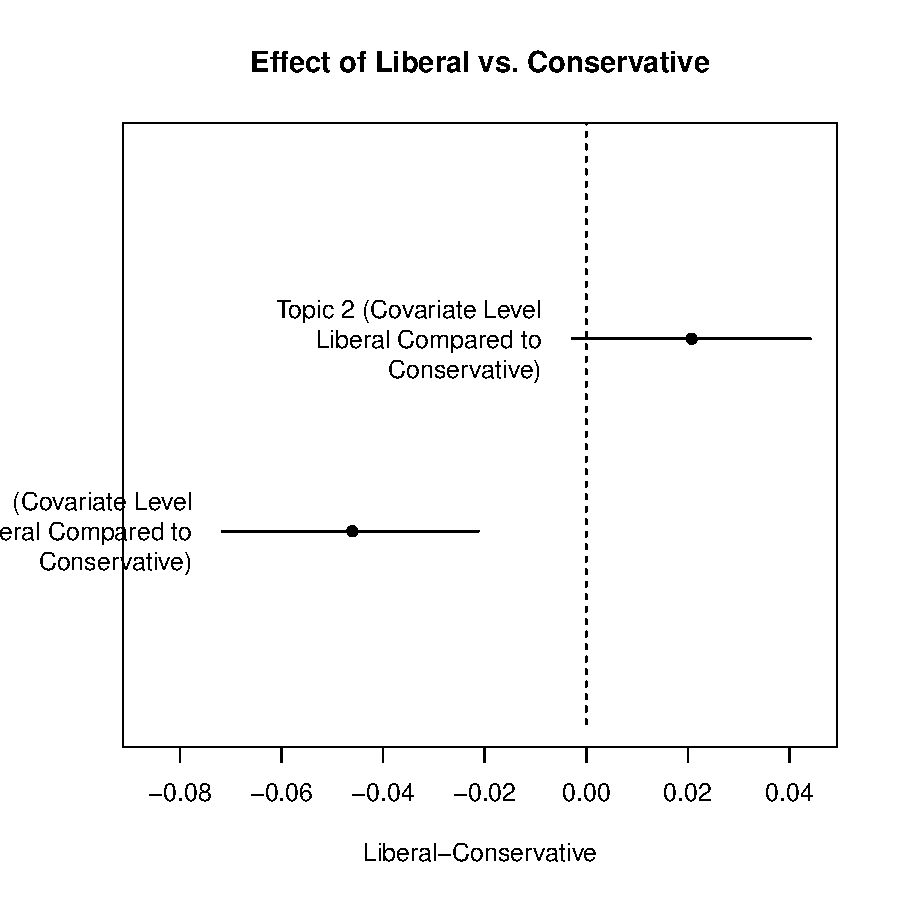
\includegraphics{stmVignette-012}
\caption{Example documents highly associated with topic 5.}
\label{fig:example}
\end{center}
\end{figure}



\subsubsection{Plotting Topic/Metadata relationships}

The \texttt{STM} package comes with a rich suite of plotting functions that lets users explore the relationship between their metadata and topical prevalence or content.

Before plotting, we have to run \code{estimateEffect} in order to simulate a set of parameters which can then be plotted.  \code{estimateEffect} uses the method of composition to calculate uncertainty in the parameters fitted by the linear model of the topic proportions on the covariates.  In the below example this is run on topics 1 and 2. \code{estimateEffect} should be run and saved before plotting because it can be time intensive to calculate uncertainty estimates and/or because users might wish to plot different quantities of interest using the same simulated parameters.\footnote{The help file for this function describes several different ways for uncertainty estimate calculation, some of which are much faster than others.} The output can then be plotted. In this example we use a string variable and it is required that for this function we that we first convert it into a factor variable.

\begin{Schunk}
\begin{Sinput}
> meta$rating<-as.factor(meta$rating)
> prep <- estimateEffect(1:2 ~ rating,poliblogPrevFit, meta=meta)
\end{Sinput}
\end{Schunk}

The syntax of the \code{estimateEffect} function is designed so users specify the set of topics they wish for estimation to be done on, and then a formula for metadata of interest. After the necessary method of composition simulations are done particular estimate strategies and standard plot design features can be used by calling the \code{plot.estimateEffect} function. First, users must specify the variable that they wish to use for calculating an effect. If there were multiple variables specified in \code{estimateEffect}, then all other variables are held at their sample median. In this example we only have one variable, "rating". Users must also select the type of quantity that is to be plotted. When the covariate of interest is binary, or users are interested in a particular contrast, the method="difference" option will plot the change in topic proportion shifting from one value to the other. Figure~\ref{fig:difference} gives an example. For factor variables, users may which to plot the marginal topic proportion for each of the levels ("pointestimate").


\begin{figure}[t!]
\begin{center}
\begin{Schunk}
\begin{Sinput}
> plot.estimateEffect(prep, "rating", model="poliblogPrevFit", method="difference",
+             cov.value1="Liberal",cov.value2="Conservative",
+            xlab="Liberal-Conservative",
+            main="Effect of Liberal vs. Conservative"
+            )
\end{Sinput}
\end{Schunk}
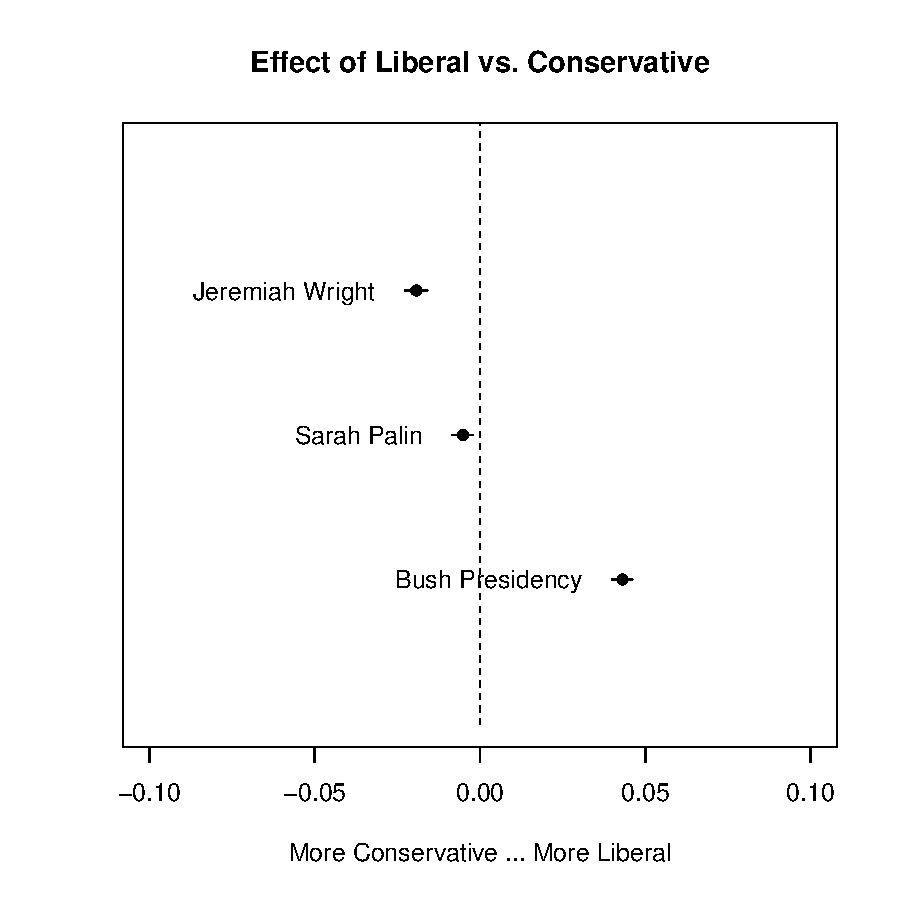
\includegraphics{stmVignette-014}
\caption{Graphical Display of Topical Prevalence Contrast.}
\label{fig:difference}
\end{center}
\end{figure}


Notice how the function makes use of standard labeling options available in the native plot() function. This allows the user to customize labels and other features of their plots. We note that in the package we leverage generics for the plot functions. As such, one can simply use \code{plot} instead of writing out the full extension (e.g., in Figure~\ref{fig:difference} one could use \code{plot()} instead of \code{plot.estimateEffect}). For expositional purposes in this vignette, we include the entire extension.

We can also plot the influence of covariates included in topical content. A topical content variable allows for the vocabulary used to talk about a particular topic to vary. First, the STM must be fit with a variable specified in the content option. In the below example, ratings serves this purpose.

\begin{Schunk}
\begin{Sinput}
> poliblogContent <- stm(out$documents,out$vocab,K=20, prevalence =~ rating,
+         content=~rating, max.em.its=75, data=meta)
\end{Sinput}
\end{Schunk}

Next, the results can be plotted using the \code{plot.STM(,type="perspectives")} function.  This functions shows which words within a topic are more associated with one covariate value versus another. In Figure~\ref{fig:perp}, vocabulary differences by ratings is plotted for topic 5.\footnote{As described in the help file for plot.stm, the perspectives option also can be used to contrast two separate topics even when no content covariate is specified.}\footnote{At this point you can only
 have a single variable as a content covariate, although that variable can have any number of groups. It cannot be continuous. Note that the computational cost of this type of model rises quickly with the number of groups and so it may be advisable to keep it small.}

\begin{figure}[t!]
\begin{center}
\begin{Schunk}
\begin{Sinput}
> plot.STM(poliblogContent,type="perspectives", topics=5)
\end{Sinput}
\end{Schunk}
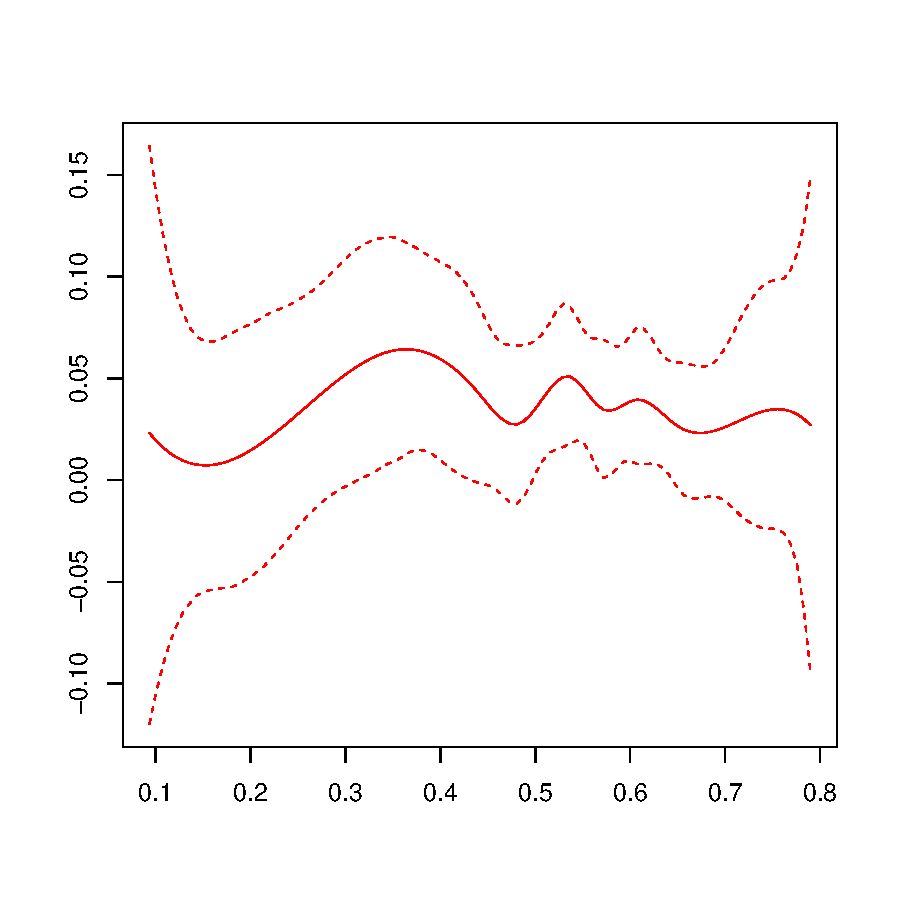
\includegraphics{stmVignette-016}
\caption{Graphical Display of Topical Perspectives.}
\label{fig:perp}
\end{center}
\end{figure}

This function can also be used to plot the contrast in words across two topics, as is shown in Figure~\ref{fig:perp2}.
\begin{figure}[t!]
\begin{center}
\begin{Schunk}
\begin{Sinput}
> plot.STM(poliblogPrevFit,type="perspectives", topics=c(5,6))
\end{Sinput}
\end{Schunk}
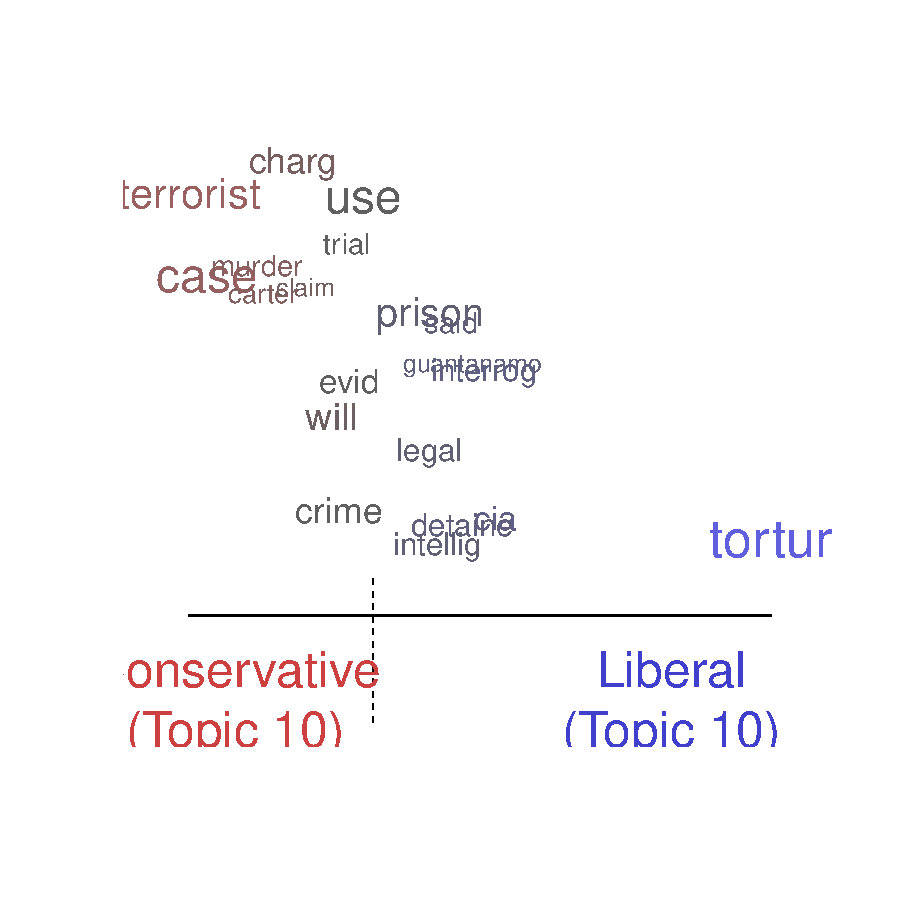
\includegraphics{stmVignette-017}
\caption{Graphical Display of Topical Perspectives.}
\label{fig:perp2}
\end{center}
\end{figure}


%We showcase this by using the data from \citet{gentzkow2010drives} that we previously loaded from the \pkg{textir} package.

In the previous example we had a single binary variable. A feature of the \code{stm()} function is that ``prevalence'' can be expressed as a formula which can include multiple covariates and factorial or continuous covariates.  For example, by using the formula setup we can enter other covariates additively. Additionally users can include more flexible functional forms of continuous covariates, including standard transforms like log() etc., as well as ns() or bs() from the splines package. The \pkg{stm} package also includes a convenience function s(x) which selects a fairly flexible b-spline basis. Interactions between covariates can also be added using the standard notation for \texttt{R} formulas. In the below example, we enter in the variables additively, but allowing for the day variable, an integer variable measuring which day the blog was posted, to have a non-linear relationship in the topic estimation stage.

\begin{Schunk}
\begin{Sinput}
> poliblogSmoothing <- stm(out$documents,out$vocab,K=20,
+         prevalence =~ rating + s(day), max.em.its=75, data=meta)
> 
\end{Sinput}
\end{Schunk}

\begin{Schunk}
\begin{Sinput}
> prep <- estimateEffect(c(17,18) ~ rating + s(day), 
+                        poliblogSmoothing, metadata=meta, 
+                        uncertainty="None")
\end{Sinput}
\end{Schunk}

After estimating the STM, researchers can investigate the relationship between topics and a particular covariate. When users have variables that they want to treat continuously, users can choose between assuming a linear fit or using splines. In the previous example, we allowed for the day variable to have a non-linear relationship in the topic estimation stage. Here we restrict effect estimation to two topics (topic 17 and 18) as well as do not propagate the full amount uncertainty which simply speeds up computational time but results in too narrow confidence intervals (\code{uncertainty="None"}). We can then plot its effect on topics in Figure~\ref{fig:spline}.

\begin{figure}[t!]
\begin{center}
\begin{Schunk}
\begin{Sinput}
> plot.estimateEffect(prep, "day", method="continuous", topics=17,
+         model=poliblogSmoothing,printlegend=FALSE)
\end{Sinput}
\end{Schunk}
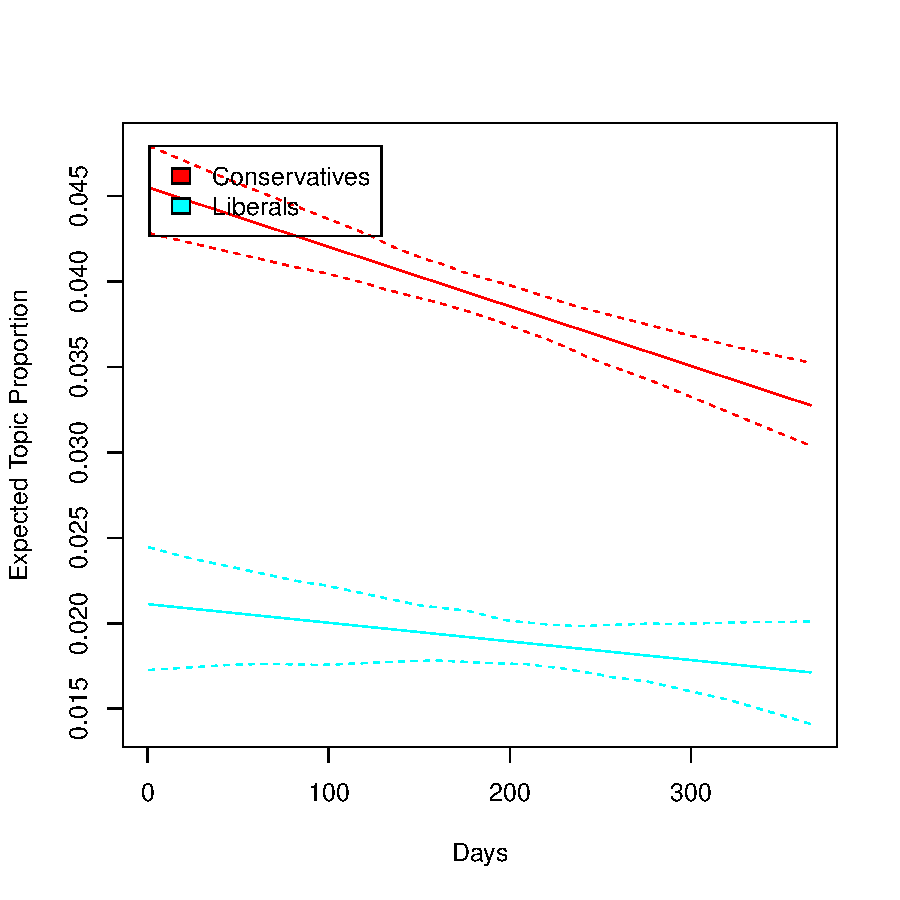
\includegraphics{stmVignette-020}
\caption{Graphical Display of Topical Content. Topic 17 prevalence is plotted as a smooth function of day, holding rating at sample median.}
\label{fig:spline}
\end{center}
\end{figure}

Another modification that is possible in this framework is to allow for interactions between covariates. In this example, we re-estimated the STM to allow for an interaction between day and ratings. Then in \code{estimateEffect()} we include the same interaction. This allows us in \code{plot.estimateEffect} to have this interaction plotted. We display the results in Figure~\ref{fig:spline2}. Note that the ability to plot interactions is somewhat limited and only supports interactions with a binary effect modification covariate, and continuous variable of interest. This will change in the near future.


\begin{Schunk}
\begin{Sinput}
> poliblogInteraction <- stm(out$documents,out$vocab,K=20,
+     prevalence =~ rating*day, max.em.its=j, data=meta)
> 
\end{Sinput}
\end{Schunk}


\begin{figure}[t!]
\begin{center}
\begin{Schunk}
\begin{Sinput}
> prep <- estimateEffect(c(7) ~ rating*day,
+         poliblogInteraction, metadata=meta, uncertainty="None")
> plot.estimateEffect(prep, covariate="day", model=poliblogInteraction,
+                  method="continuous")
\end{Sinput}
\end{Schunk}
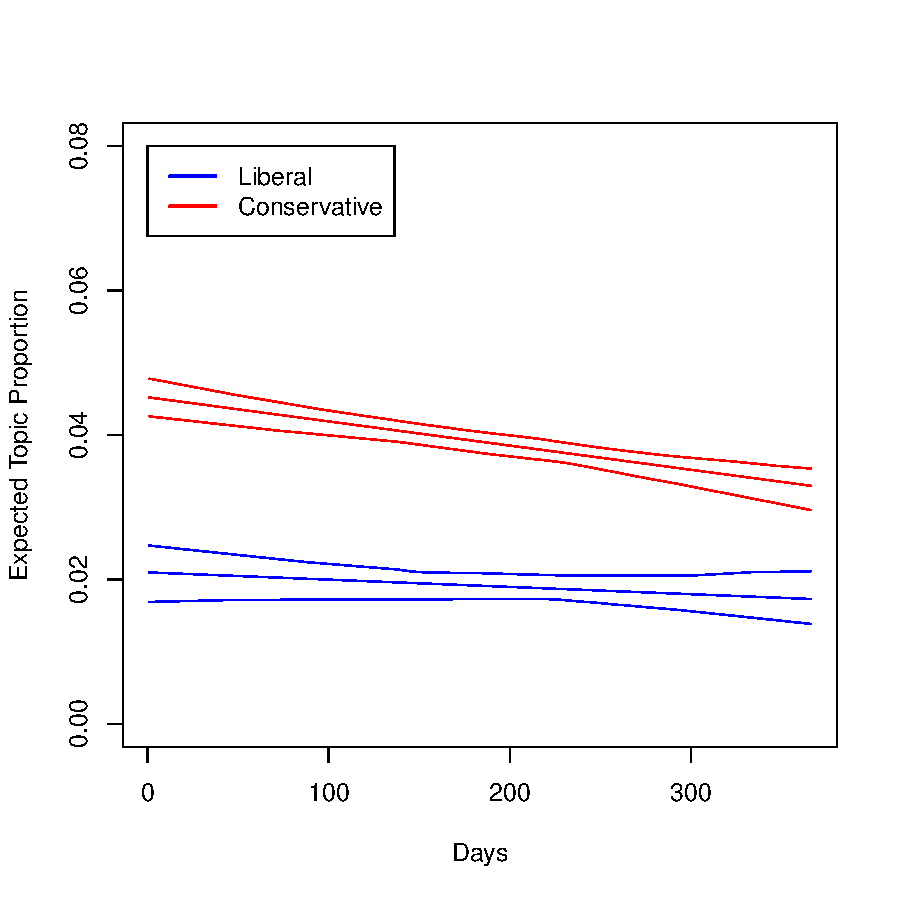
\includegraphics{stmVignette-022}
\caption{Graphical Display of Topical Content allowing for interaction between day of blog post and liberal versus conservative interaction. Topic 7 prevalence is plotted as linear function of day, holding the rating at either 0 (Liberal) or 1 (Conservative). Were other variables included in the model, they would be held at their sample medians.}
\label{fig:spline2}
\end{center}
\end{figure}


More details are available in the help file for this function.\footnote{An additional option is the use of local local regression (loess). In this case, because multiple covariates are not possible a separate function is required, \code{plotTopicLoess}, which contains a help file for interested users.}.


\subsubsection{Corpus level plotting}

Corpus level visualization can be done in several different ways. The first relates to the expected proportion of the corpus that belongs to each topic. This can be be plotted using \code{plot.stm(,type="summary")}. An example from the political blogs data is given in Figure~\ref{fig:summary}.

\begin{figure}[t!]
\begin{center}
\begin{Schunk}
\begin{Sinput}
> plot.STM(poliblogPrevFit,type="summary")
\end{Sinput}
\end{Schunk}
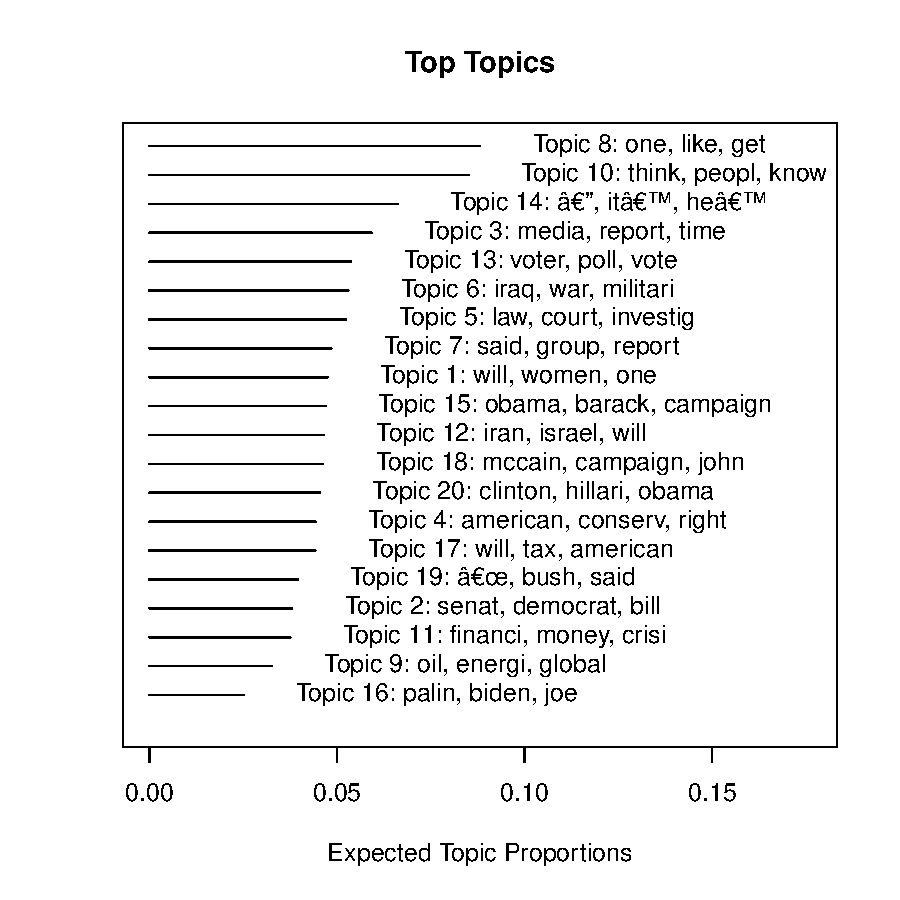
\includegraphics{stmVignette-023}
\caption{Graphical Display of Estimated Topic Proportions.}
\label{fig:summary}
\end{center}
\end{figure}

Users can also plot features of the corpus as a whole. First, the Structural Topic Model permits correlations between topics. Positive correlations between topics indicate that both topics are likely to be discussed within a document. These can be visualized using \code{plot.topicCorr()}. The user can specify a correlation threshold.  If two topics are correlated above that threshold, than those two topics are considered linked.  After calculating the links between topics, \code{plot.topicCorr} produces a layout of topic correlations using a force-directed layout algorithm. \code{plot.topicCorr} has several options that are described in the help file.

\begin{Schunk}
\begin{Sinput}
> mod.out.corr<-topicCorr(poliblogPrevFit)
\end{Sinput}
\end{Schunk}

\begin{figure}[t!]
\begin{center}
\begin{Schunk}
\begin{Sinput}
> plot.topicCorr(mod.out.corr)
\end{Sinput}
\end{Schunk}
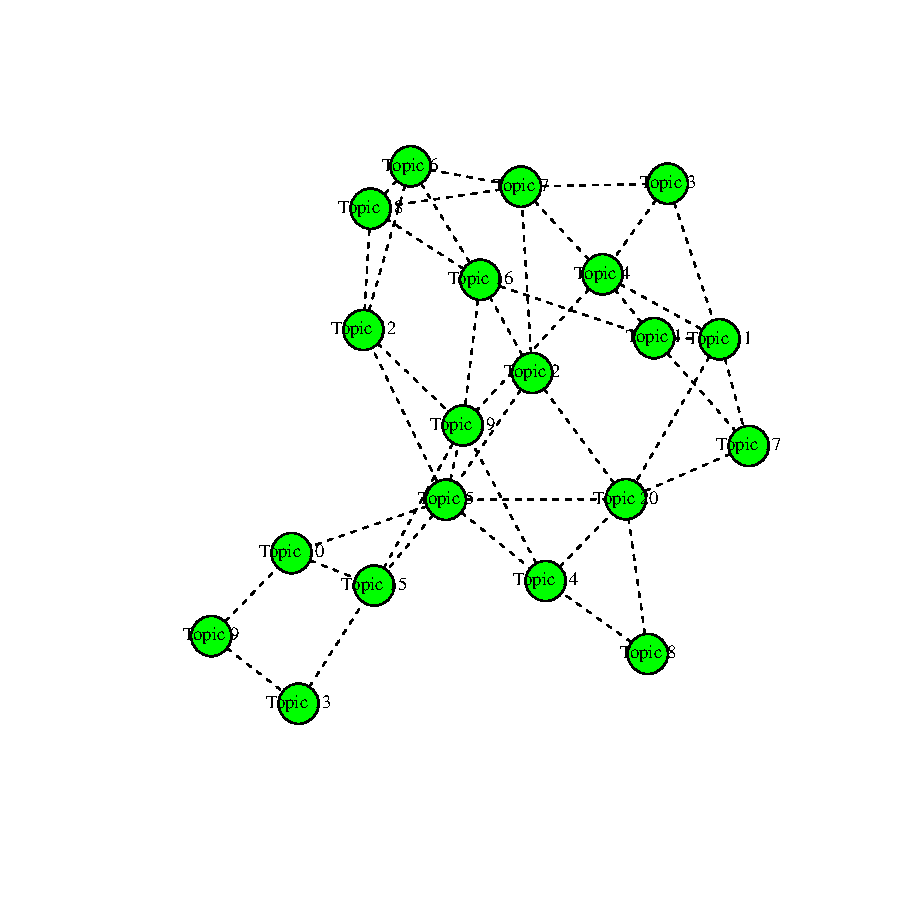
\includegraphics{stmVignette-025}
\caption{Graphical Display of Topic Correlations.}
\label{fig:correlations}
\end{center}
\end{figure}





\section{Changing Basic Estimation Defaults}
In this section we briefly overview how to change details of estimation that may be of interest to advanced users.

\subsection{Convergence Criteria}
Estimation in the STM proceeds by variational EM.  Convergence is controlled by relative change in the variational objective.  Denoting by $\ell_t$ the approximate variational object at time $t$, convergence is declared when the quantity $\ell_t - \ell_{t-1}/$abs($\ell_{t-1}$) drops below tolerance.  The default tolerance is 1e-5 by default and can be changed using the \code{emtol} argument.

The argument \code{max.em.its} sets the maximum number of iterations.  If this threshold is reached before convergence is assessed a message will be printed to the screen.  The default of 100 iterations is simply a general guideline.

Once a model has been fit, convergence can easily be assessed by plotting the variational bound as in Figure \ref{fig:converge}. 

\begin{figure}[t!]
\begin{center}
\begin{Schunk}
\begin{Sinput}
> plot(poliblogPrevFit$convergence$bound,type="l", ylab="Approximate Objective",
+     main="Convergence")
\end{Sinput}
\end{Schunk}
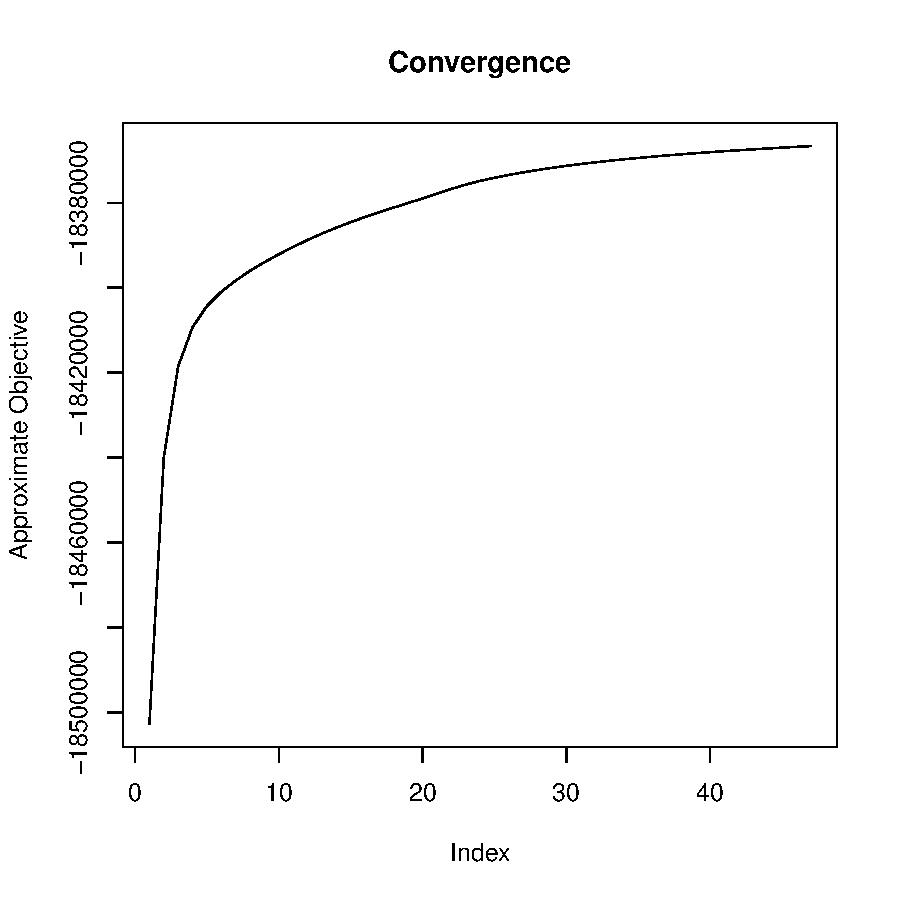
\includegraphics{stmVignette-026}
\caption{Graphical Display of Convergence.}
\label{fig:converge}
\end{center}
\end{figure}

Additionally convergence can be specified in terms of the number of iterations without change in the most probable words.  See the documentation for \code{stm} for more information.

\subsection{Initialization}
As with any EM based estimation strategy, starting values are required. In order to change how starting values are chosen, the argument \code{init.type} has several different options including \code{LDA}, \code{DMR} (Dirichlet Multinomial Regression Topic Model), and \code{Random}).
\code{LDA} is the default and uses a few passes of collapsed Gibbs sampling for the standard LDA model as an initializer.  This tends to provide a fairly good starting region.  Random initializations often start with a dramatic lower value of the objective function but also recover quite quickly.

\subsection{Reporting}
The default is to have the status of iterations print to the screen. The \code{verbose} option turns printing to the screen on and off.

DUring the E-step the algorithm prints one dot for every $1\%$ of the corpus it completes and announces completion along with timing information.  Printing for the M-Step depends on the algorithm being used.  For models without content covariates M-step estimation should be nearly instantaneous.  For models with content covariates and the Jeffreys prior, the algorithm prints one dot for each parameter vector update (thus for K=10 topics, and a 2-level covariate with interactions you will see 32 dots per M-step pass).  

By default every 5th iteration will print a report of top topic and covariate words.  The \code{reportevery} option sets how often these reports are printed.

Finally the \code{keepHistory} option can be used to save the entire parameter history at each EM iteration.  This can be useful for diagnostic purposes but note that when the number of words in the vocabulary, the number of documents or the number of topics is large, the history can quickly overwhelm available active memory. Thus we recommend leaving the default of \code{FALSE} in most cases.


\subsection{SAGE}
The Sparse Additive Generative (SAGE) model conceptualizes topics as sparse deviations from a corpus-wide baseline \citep{eisenstein2011sparse}.  While computationally more expensive this can sometimes produce higher quality topics .  Whereas LDA will tend to assign rare words exclusively to one topic, the regularization of the SAGE model ensures that words only load onto topics when they have sufficient counts to overwhelm the prior.  In general this means that SAGE topics will tend to have fewer words that distinguish them from other topics, but those words are more likely to be meaningful.  Importantly for our purposes the SAGE framework makes it straightforward to add covariate effects into the content portion of the model. 

\paragraph{Covariate-Free SAGE}
While SAGE topics are enabled automatically when using a covariate in the content model they can also be used even without covariates.  To activate SAGE topics simply set the option \code{LDAbeta=FALSE}.

\paragraph{Covariate-Topic Interactions}
By default when a content covariate is included in the model, we also include covariate-topic interactions.  In our political blog corpus for example this means that the probability of observing a word from a Conservative blog in Topic 1 is formed by combining the baseline probability, the Topic 1 component, the Conservative component and the Topic 1 - Conservative interaction component.

Users can turn off interactions by specififying the option \code{interactions=FALSE}.  This can be helpful in settings where there isn't sufficient data to make reasonably inferences about all the interaction parameters.  It also reduces the computational intensity of the model.

\section{Alternate Priors}
In this section we overview options for altering the prior structure in the \code{stm}  function.  We highlight the major alternatives and refer interested users to the documentation for additional details.

\subsection{Changing Estimation of Prevalence Covariate coefficients}

The user can choose between two options: "Pooled" is the default and estimates a model where the coefficients on topic prevalence have a zero-mean Normal prior with variance given a broad
 inverse-gamma hyperprior.

You can also choose \code{gamma.prior="L1"} which uses the \code{glmnet} package \citep{friedman2010regularization} to allow for grouped penalties between the L1 and L2 norm. In these settings we estimate a regularization path and then select the optimal shrinkage parameter using a user-tuneable information criterion. By default selecting the L1 option will apply the L1 penalty selecting the optimal shrinkage parameter using AIC. The defaults have been specifically tuned for the STM but almost all the relevant arguments can be changed through the \code{control} argument. Changing the \code{gamma.enet} parameter by specifying \code{control=list(gamma.enet=.5)} allows the user to choose a mix between the L1 and L2 norms. When set to 1 (as by default) this is the lasso penalty, when set to 0 its the ridge penalty. Any value in between is a mixture called the elastic net.  

Because the penalties are grouped covariates will tend to influence all topics are none.  Thus this option is best employed in settings where the analyst has a large number of covariates but expects most of them to have no effect.

\subsection{Changing Covariance Matrix Prior}
The \code{sigma.prior} argument is a value between 0 and 1 defaulting to 0.  The update for the covariance matrix is formed by taking the convex combination of the diagonalized covariance and the MLE with weight given by the prior.  Thus by default we are simply maximizing the likelihood.  When \code{sigma.prior=1} this amounts to setting a diagonal covariance matrix.  This argument can be useful in settings where topics are at risk of becoming too highly correlated.  However, in extensive testing we have come across very few cases where this was needed.

\subsection{Changing the Content Covariate Prior}
The \code{kappa.prior} option provides two sparsity promoting prios for the content covariates.  The default is \code{kappa.prior="Jeffreys"} and uses a scale mixture of Normals where the precisions $\tau$ are given improper Jeffreys priors $1/\tau$.  

Specifying the option \code{kappa.prior="L1"} uses \code{glmnet} to impose a penalty between the L1 and L2 norm (as controlled by the \code{control} parameter \code{kappa.enet}).  In general we strongly recommend keeping close to the L1 norm as sparsity is important for estimation.

When choosing the \code{L1} option, the user can also choose whether to fix the word probability intercept to the empirical log probability or estimate it freely.  It is fixed by default but can be changed by setting the control option \code{control=list(fixedintercept=FALSE)}.  

There are over a dozen additional options documented in \code{stm} for altering additional components of the prior, most of them focusing on the content covariate model.  

\section{Conclusion}

The  \pkg{stm} package provides a flexible integration of document metadata and topic modeling. This vignette provides an overview of use and features. We encourage users to consult the extensive help files for more details, as well as read the companion papers that illustrate the application of this method.

\clearpage
\pdfbookmark[1]{References}{References}
\bibliography{vignetteBib}


\end{document}





%\subsection{Basic Models}
\begin{comment}
As before we can estimate a model with no covariates to recover the Correlated Topic Model
 (see Blei and Lafferty 2006). Here we set the number of topics to 5.
\begin{Schunk}
\begin{Sinput}
> mod.out <- stm(documents,vocab,K=5, max.em.its=5)
\end{Sinput}
\end{Schunk}

The structure of the output can be investigated. Most of the necessary information is at the top of the returned object.
\begin{Schunk}
\begin{Sinput}
> str(mod.out,1)
\end{Sinput}
\end{Schunk}

The STM package comes with a range of helper functions that we review next.
\end{comment}



\begin{comment}
Covariates for the content model are also specified via formula.  At this point you can only
 have a single variable although that variable can have any number of groups. It cannot be continuous. Note that the computational cost of this type of model rises quickly with the number of groups and so it may be advisable to keep it small.

\begin{Schunk}
\begin{Sinput}
> mod.out <- selectModel(documents,vocab, K=10,
+                prevalence= ~party, data=metadata,
+                content=~party, runs=3)
> plotModels(models)
\end{Sinput}
\end{Schunk}
\end{comment}

\begin{comment}
\section{Plotting and Visualization}

For additional discussion of options for plotting and visualization, please see the help files.

\begin{Schunk}
\begin{Sinput}
> ?ploteffect()
> ?prep.plot()
> ?plot.stm()
> ?plottopics()
> ?plotquote()
\end{Sinput}
\end{Schunk}
\end{comment}



\begin{comment}
\subsubsection{Estimation with no prevalence parameter}
When not topical prevalence model is included, the stm returns the results from the correlated topic model (see Blei and Lafferty 2006).

In this example, we are estimating the correlated topic model with 5 topics.
\begin{Schunk}
\begin{Sinput}
> mod.out <- stm(poliblog.documents,poliblog.vocab,K=5,
+                max.em.its=3,verbose=FALSE)
\end{Sinput}
\end{Schunk}



As before we can quickly look at the results using the \code{labeltopics()} function. Users can also explore relationships of the output to metadata, but in this case users might ask themselves why they did not include these covariates directly as a topical prevalence parameter.

\begin{Schunk}
\begin{Sinput}
> labelTopics(mod.out,n=3)
\end{Sinput}
\begin{Soutput}
Topic 1 Top Words:
 	 Highest Prob: house, democrats, said 
 	 FREX: house, republicans, senate 
 	 Lift: house, pelosi, republicans 
 	 Score: house, republicans, democrats 
Topic 2 Top Words:
 	 Highest Prob: obama, mccain, said 
 	 FREX: wright, fox, church 
 	 Lift: wrights, wright, ayers 
 	 Score: obama, mccain, wright 
Topic 3 Top Words:
 	 Highest Prob: president, bush, tax 
 	 FREX: tax, oil, trade 
 	 Lift: oil, prices, trade 
 	 Score: tax, president, oil 
Topic 4 Top Words:
 	 Highest Prob: day, political, state 
 	 FREX: law, book, court 
 	 Lift: diaries, rangers, thread 
 	 Score: law, day, state 
Topic 5 Top Words:
 	 Highest Prob: clinton, obama, voters 
 	 FREX: delegates, primary, carolina 
 	 Lift: precincts, delegates, rasmussen 
 	 Score: clinton, obama, voters 
\end{Soutput}
\end{Schunk}
\end{comment}



\begin{comment}
We begin with a simple model where we have a single covariate for topic prevalence and have specified 10 topics.
\begin{Schunk}
\begin{Sinput}
> mod.out <- stm(documents,vocab, K=10,
+                prevalence= ~party, data=metadata,max.em.its=5)
\end{Sinput}
\end{Schunk}
\end{comment}

\begin{comment}

\begin{Schunk}
\begin{Sinput}
> length(poliblog.documents) #there are 773 documents
\end{Sinput}
\begin{Soutput}
[1] 773
\end{Soutput}
\begin{Sinput}
> length(poliblog.vocab)     #and 1290 items in the vocab
\end{Sinput}
\begin{Soutput}
[1] 1290
\end{Soutput}
\end{Schunk}

\end{comment}
